\documentclass[12pt]{article}
\usepackage[utf8]{inputenc}
\usepackage{amsmath}
\usepackage{mathrsfs}
\usepackage{amssymb}
\usepackage{amsfonts}

\DeclareMathOperator{\logit}{logit}
\DeclareMathOperator*{\argmax}{arg\,max}
\DeclareMathOperator*{\argmin}{arg\,min}
\newcommand{\red}[1]{\textcolor{red}{#1}}
\newcommand{\blue}[1]{\textcolor{blue}{#1}} 

\usepackage[
    a4paper,
    left = 2.5cm,
    right = 2.5cm,
    top = 2.5cm,
    bottom = 2.5cm
]{geometry}

\usepackage{graphicx}
\usepackage{booktabs}
\usepackage{placeins}
\usepackage[headings]{fullpage}
\usepackage{xcolor}
\usepackage{hyperref}
\usepackage{fancyhdr}
 %For aligned formulas
 \usepackage{IEEEtrantools}
\usepackage{listings} %Source code listings https://en.wikibooks.org/wiki/LaTeX/Source_Code_Listings

% \lstset{
%     language=R, %You can always set to another language
%     breaklines,
%     deletekeywords={category},
%     basicstyle=\ttfamily\footnotesize,
%     otherkeywords={!,!=,~,\$,*,\&,\%/\%,\%*\%,\%\%,<-,<<-},
%     literate={~}{$\sim$}1 {<-}{{$\gets$}}1
% }

\usepackage[
    backend=biber,
    style=apa,
    maxcitenames=2,
    mincitenames=1,
    sorting=ynt
    ]{biblatex}
\addbibresource{bibfile.bib}

\setlength{\headheight}{15pt}
\pagestyle{fancy}
\fancyhf{}
\rhead{Odole, Cunha, and Murthy} % Fill in your name
%\lhead{Bayesian Statistics \& Probabilistic Machine Learning---Project Report}
\rfoot{Page \thepage}


\begin{document}

\begin{titlepage}
        \centering % Center all text
        \vspace*{\baselineskip} % White space at the top of the page
        
        {\huge YOUR TITLE}\\[0.2\baselineskip] % Title
        
        
        \vspace*{\baselineskip}
        
        {\Large --- Project Report ---\\
          Advanced Bayesian Data Analysis\\[\baselineskip]} % Tagline(s) or further description
        \vspace*{\baselineskip}
        
        {\LARGE Eldaleona Odole,  Leonor Cunha, and Anarghya Murthy\\[\baselineskip]} % Editor list  
        
        \vspace*{\baselineskip}

        \vfill
        
        \today \par % Location and year
        
        \vspace*{\baselineskip}

        {\itshape TU Dortmund University\par} % Editor affiliation
    \end{titlepage}

\clearpage

% \section{Template}
% This is a template for the project report in the course Advanced Bayesian Data Analysis.
% Fill in your title and names for the title page and header and follow the general structure. You don't have to use multiple chapters or sections at all for this short report, but if you do, don't go further than subsections--- \textcite{feynman1963lnphysics} didn't need to\ldots

% Some examples on how to use \LaTeX{} are shown below. If you want to reference something, you can do it as so:
% \textcite{mcelreath2016statistical}.

% \subsection{Images}
% \begin{figure}
%     \begin{center}
%     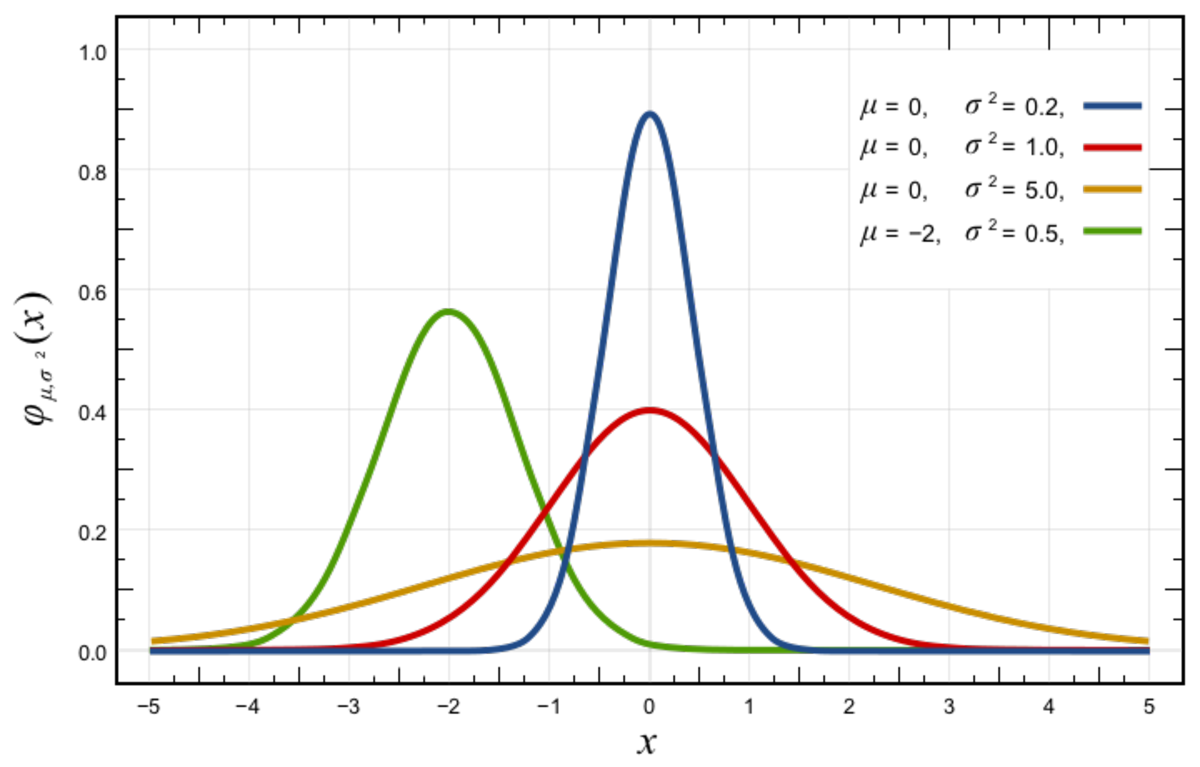
\includegraphics[width=0.5\textwidth]{figures/Normal_Distribution_PDF.pdf} %try to never force a figure placement
%     \caption{Probability density function for the Normal distribution. The red curve is the standard normal distribution. [By Inductiveload - self-made, Mathematica, Inkscape, Public Domain, \url{https://commons.wikimedia.org/w/index.php?curid=3817954}]}
%     \label{fig:normal_sample}
%     \end{center}
% \end{figure}

% This is an example for how to insert images into your document. When talking about a figure, you should always point out which one you mean, i.e., ``As you can see in Figure~\ref{fig:normal_sample}.''

% \subsection{Tables}
% A table has a caption \textit{above} the table as in Table~\ref{tab:my_label}.

% \begin{table} %You can place [h] immediately after \begin{table} to force the placement of the table. Generally speaking never do that---LaTeX usually places them in a sane way!
%     \centering
%     \caption{My caption.}
%     \label{tab:my_label}
%     \begin{tabular}{c|l} % l, r, and c justified inside cells.
%         \hline
%          Poisson & $\lambda$ \\ % Always end a line with \\
%          Normal &  $\mu$ and $\sigma$\\ 
%         \hline
%     \end{tabular}
% \end{table}

% \subsection{Formulas}
% This is a small example for how to include formulas into your document. $a^2 + b^2 = c^2$ will inline a formula, while
% $$c \leq a + b$$
% will give the formula its own line.

% \subsection{Formulas}
% You also might want to write out models:

% {\footnotesize % you align formulas using & 
% \begin{IEEEeqnarray*}{rCl}
% \mathrm{L}_i & \sim & \mathrm{Binomial}(n_i,p_i)\\
% \mathrm{logit}(p_i) & = & \alpha_{\mathrm{SUBJECT}[i]} + (\beta_P + \beta_{PC}C_i)P_i\\
% \alpha_{\mathrm{SUBJECT}} & \sim & \mathrm{Normal}(0,10) \\
% \beta_P & \sim & \mathrm{Normal}(0,10)\\
% \beta_{PC} & \sim & \mathrm{Normal}(0,10)
% \end{IEEEeqnarray*}
% }


% \subsection{Source code}
% Of course, formatting source code is always nice.
% \begin{lstlisting}
% m <- map(
%     alist(
%         height ~ dnorm(mu, sigma),
%         mu <- a + b*weight,
%         a ~ dnorm(0, 100),
%         b ~ dnorm(0, 10),
%         sigma ~ dunif(0, 50) 
%     ), 
%     data=d2)
% \end{lstlisting}

% \subsection{Math fonts}
% Different math fonts are also available to you:

% $\mathrm{ABCDE abcde 1234}$

% $\mathit{ABCDE abcde 1234}$

% $\mathnormal{ABCDEabcde1234}$

% $\mathcal{ABCDE abcde 1234}$

% $\mathscr{ABCDE abcde 1234}$

% $\mathfrak{ABCDE abcde 1234}$

% $\mathbb{ABCDE abcde 1234}$



\thispagestyle{empty} % Prevents the header and footer from being displayed on the title page
\newpage

\tableofcontents
\newpage


\section{Introduction}


\textcolor{red}{notes to ourselves about things that should go in each section can be in red like this so we dont forget to delete them :)}


\subsection*{Background}
The association between a voters demographics (gender, age, education etc.) and their propensity to vote for either a democratic or republican candidates is a topic of extensive study. The large political polling organization such as Gallup and Pew Research tend to analyze their polls by breaking respondants into smaller demographic groups \red{cite}. However, less is known about the relationship between voting outcomes and the voter's environment. Our modeling would like to investigate the conventional wisdom that says cities tend to be more progressive. To put it more concretely we want to investigate the question; "How does urbanization of a particular US House distrcit affect the resulting party that is elected?". 

To answer our question about the nature of the relationship between urbanizaiton and partisan voting outcomes, we choose to investigate the 2022 House Election. Every two years the United States elects 435 officials to the House of Representatives. Each state is allocated one of the the 435 House seats with the rest being allocated roughly proportional to the share of total population living in each state \red{cite}. We then use each of the districts as a single replicate. 

The 2022 House Election takes places during a non-presidential year, and is the most recent election following the 2020 Census and redistricting, allowing us to use the most recently available district maps, and demographic data. Within this report we combine demographic data and urbanization data into a logistic regression model to predict the district voting outcomes of the 2022 House Election. 

% Previous attempts? 

\subsection*{comparative literature}
Inherent in our analysis is the assumption that repuclican and democratic voters are not evenly distributed, rather we assume that the distribution of voters is informative for our analysis. Much of the current research related to the relationship between urbanization and partisan voting focuses on the practice of gerrymandering. Gerrymanding is practice of redrawing the voting district boundaries in favor of a particular political party. We ignore the impact of gerrymandering in our analysis, since the method of determining if a distict has been gerrymandered is rather unclear and out of the scope of this project.

Since we are using a custom curated dataset, there exists no directly comparableresearch, however we did find interesting ideas related to urbanization and partisianship. One example of this would be the idea of the inefficent distribution of Democrats in cities, as explored by \textcolor{red}{CITE}. In their analysis they discuss the phenomena of spatial inefficency wherein higher concentrations of democratic voters in urban areas leads to fewer districts voting for democratic candidates that would be expected. Rather than trying to predict the partisan outcome of a particular district, their analysis focuses on measuring partisan spatial efficency in order to understand the impact of gerrymandering \red{CITE}. 

Although the authors in \red{cite title} look at election outcomes through the lense of spatial efficency and we are trying to look at election results of districts with respect to their urbanizaition, we can take the following insights from their analysis. First the distribution of Democrats and urbanization are inexplicably linked, they found that all over the country Democrats tend to be concentrated in urban areas which indicate that it will likely be a good predictor. We would like to investigate to what extent that is true. They also note that the effect of spatial efficency is highly dependent on state and the branch of goverment. When considering that urbanization can be considered a proxy for spatial inefficency, this further supports our decision to model urbanindex hierachically. 
% points to something ... 

\red{why this particular modeling approach? Also what was our modeling approach?}

\subsection*{model approach/motivation}
\subsubsection*{Two party system}

\red{why not shift this to the data section?}
\textcolor{red}{Leonor: here is an explaination for it being two parties, kinda long but yeah}
Although technically a multiparty system, the U.S. is often called a two party system due to the domination of the major political parties the Democrats and Republicans \textcolor{red}{(cite)}. These parties dominate particularly on the fedral level because political candidates are required to get a plurality of votes rather than a majority of votes which the two largest parties often reach. This is further reinforced as would be third-party voters, often vote for one of the two major parties so ensure their voice is heard, rather than using thier vote on a candidate unlikely to reach a plurality of votes \textcolor{red}{(cite)}. Within our dataset, there are no districts represented by a third-party candidate and as such we will refer to the U.S. as being a two party system, which led to using logistic regression as a natural choice for modeling.  \red{i would say led to modeling winner as a binary variable, this doesnt necessarily lead to logistic regression}

% This is related to our analysis because where these authors were trying to understand the outcomes as related to distribution of voters within a city we are tyring to do somehting similar but rather look to predicting the outcomes of particular districts with respect to their level of urbanization. Whereas the authors assume some sort of causal mechanism in the urbanization being a determinate variable for partisanship be assume rather that both partisanship and urbanization are independent given some other third latent variable. 

% They call this phenomena partisan , which happens because the districts drawn in cities te that tend to more often be located quite densly in the urban core and  Republicans tend to live further from city centers .




\textcolor{red}{this is something like assumptions but im not really sure what to say}
Since the districts are allocated based on population, they are approximately the same size, which allows us the make the assumption the differences in voting behavior have something do with people within the districts rather than simply the size of each district. This also allows us the make exchangability assumptions with respect to state and region.

\blue{maybe put assumptions here? like the exchangability assumption?}
\red{i think model assumptions belong in the model section, at least the explanation (we can just mention the name here is it is important to)}


\section{Dataset}
Our dataset was made by combining four independent datasets related to the 2022 House election. The first dataset is the publically available urbanization dataset published by fivethirty eight from which we incorporate the variables urbanization index  and (urban) grouping into our final dataset \cite{urbanizationdataset}. From the description of the dataset: "The urbanization index is calculated as the natural logarithm of the average number of people living within a five-mile radius of every census tract in a given district, based on a weighted average of the population of each census tract. The population of a census tract is according to 2020 census data. This provides a numerical value for how urban or rural a district is. " \cite{urbanizationdataset}. The urbanization dataset was put together by FiveThirtyEight as part of their analysis  \textit{The Republican Path To a House Majority Goes Through The Suburbs} which gave election predictions leading up to the 2022 U.S. Congressional Eleciton \cite{538urbanizationarticle}. The other variable we included in our curated dataset was urban grouping, which is a collapsing of the urban index into catagories ranging from urban to rural. We however did not end up including this in our model.


The second dataset used in our analysis the Election Results Dataset from FiveThirtyEight \cite{electionresultsdataset}. It is a continuously updated repository of United States Govenor, Congressional and Presidential elections. As this dataset includes all elections going back to 1998, we only used a subset of the data relevant to the 2022 House Election. From this dataset we used the party, state, and winning party variables, it also included the variable incumbent party, which we considered also using, but the data from incumbent party is partially incomplete and would likely have very high correlation with the our target variable winning party, leading to a model that relies most heavily on incumbent party. Since we are more interested in the relationship between our model and our choose covariates we therefore decided not to include it.  

The third data used in our analysis is a subset of the 2022 American Commuity Survey Data. The American Community Survey is a yearly survey collecting information about the occupations, education attainment, income and other demographic information carried out by the United States Census Bureau. The United States Census Bureau provides an online tool to access its extensive survey database, which can then be filtered and refined for further analysis. For our analysis we included the following variables for each House district in our curated dataset; total population, percentage women, median household income, mean household income, percentage retirees, percentage bachelors degree holders above the age of 25 years old and unemployment rate among those above the age of sixteen. 

From these covariates we hoped to capture education, income, and, demographic make-up  of the districts because we thought they might be influential in determining partisan voting outcomes. However not all of these covariates were included in our final models. As previously explained, the districts are drawn in such a way that the total population of each district should be approximately the same \blue{cite}, so while this does help support our exchangability assumption, we determined that total population itself would be an unsuitable covariate. Although we intially thought that percentage women may also be a poor predictor-since women should be evenly distributed throughout the United States-however a Pew Research Survey found that women tend to lean more democrat and have higher turnout, which is why we then included it in our largest model. \blue{cite}. We also initially thought that median and mean income could be combined to as a measure of inequality, but found a study saying that inequality is not a good voting indicator on its own \blue{cite}. For that reason we choose to use only the median household income as it would be less skewed. Similarly unemployment is not a good indicator on its own, rather when unemployment is high the incumbent is more likely to loose regardless of party\blue{cite}.  We also decided to use percentage retirees instead of median age, as they were highly correlated and median age also includes a part of the population that cannot vote. 
\blue{ Why is pct retirees included in every single one of our models? }


The fourth dataset was the region dataset, which was put together manually by us following the four statistical region designations of United States Census Bureau. \textcolor{red}{Cite: First link on wiki list of regions of us }

% Our process in choosing which variables to choose then was matter of both process of elimination as well as positive testing. This process essentially worked in two ways, first we tried to determine the relationship between voting outcomes and a particular factors based on political science research. From the remain vaiables we then looked at different testing strategies for which covariates produced highly accurate prediction results.

\subsection*{Data Cleaning}

 \blue{how did we code our variables? }
We then merged these four datasets to created our own curated dataset. We did this by merging the different datasets on shared variables. As previously said, each observation represents a particular house district, so for the first three datasets, we simply merged them based on their state and district number. To include the regions we simply used the state variable for each district. 

\red{maybe talk about the funny shit with alaska and preference voting (?)}
In the election results dataset, we encountered one instance of missing data. For all of the districts in Louisiana, the winning party was not recorded. There was however the incumbant party recorded  in the Election Results dataset and by cross referencing this with public record we found for the 2022 House Election only candidates from the incumbant party remained in each of the districts. Therefore as is reflected in our code base we used the data from the incumbant party in place of winning party for the state of Louisiana. For all other states and disticts we did not encounter this problem. 

In terms of scaling we wanted all the variables to be on roughly the same scale to aid in convergence times. In order to do that we roughly scaled median income and total population by dividing total population by one million and dividing median income by one hundred thousand. This brought each of these to roughly the same scale as the other variables. Similarly we decided to scale all of the percentage variables to be on the scale zero to one hundred rather than zero to one to make their coefficents more interpretable.  

% \subsection{Covariate Choice}

% In addition to our main variable of interest, \textit{urbanindex} we had many covariates to choose from, not all of which ended up being used in our final models. There were also many more covariates that were present in our three datasets, however we decided to drop many of them as they were not relevant to our analysis. To create our initial list of covariates, we choose variables that we thought would capture education, income, or demographic make-up  of the districts because we thought they might be influential in determining partisan voting outcomes. How we choose our final covariates was a combination of domain knowledge and initial testing. Our intial list of covariates included:

% As previously explained, the districts are drawn in such a way that the total population of each district should be approximately the same \blue{cite}, so while this does help support our exchangability assumption, we determined that total population itself would be an unsuitable covariate. 


% To then build some knowledge into our models, we looked into different qualitative studies about voting behavior, which helped guide our final choices of covariates. 



\section{Models}

%To describe our approach we wanted to test different models that incorporate the geographical hierarchy into the model. We made several common assumptions for the the four models that we compared with addtional more specific assumptions for each model. The first common assumption we made was that district voting outcomes can be modeled via logistic regression. This assumption gets at the basic logic of our models. As we said previously the outcomes of any particular district electoral race is binary (democrat/republic) so it is most appropriate to choose a modeling technique that can model binary outcomes. 
%
%\textit{Why did we choose logisitic regression?}
%
%We then moved on to our assumptions about the parameters of the linear regression model within the logistic regression model. We also assume that geography is a characteristic of each district that can be modeled hierarchical. For that reason we assume that each district is exchangeable within each state and that each state is exchangeable within each region. We assume this because for complicated historical reasons certain regiions of the united states are more similar to eachother than others. For example the Southern United states tends to be more religious and religous people tend to vote more conservatively, as a result the parameter associated with region would likely be smaller or more negative as compared to other regions. 
%We also are assuming that in some regions the value of urban index is more informative than others, the logic being that a city in a rural area will likely have stronger signal than an city among a bunch of other cities. 
%
%We also 
%
%++++++++++++++++++++++++++++++++++++++++++++

The Winning party in each congressional district race ($y_{i,j,k}$ for district $i$, state $j$, region $k$) can be modeled as the outcome of Bernoulli trial, since this is a binary variable: 
\begin{equation}
	y_{i,j,k} \sim Ber \left( \pi_{j,k} = logit^{-1}(\theta_{j,k})  \right)
\end{equation}
with probability of a Democrat win $\pi_{j,k}$ modeled as the inverse logit transform of $\theta_{j,k}$, a linear combination of our covariates. The inverse logit function converts real numbers into quantities between 0 and 1, and is therefore a standard way to model probabilities \textcolor{red}{cite}.


We tested four different models for $\theta_{j,k}$, which include different covariates in addition to our variable of interest (Urban index) and incorporate our data's hierarchical structure in different ways. Therefore, all four are Multilevel Bayesian (Logistic) Models, which require particular assumptions: \textcolor{red}{CITE} 
first, that a logistic regression accurately represents the relationship between the log-odds of a Democrat win and the explanatory variables, that is, $\theta_{j,k}$ and our covariates are linearly related; second, interchangeability, meaning that each district is exchangeable within each state and each state is exchangeable within each region; and third, that the value of urban index (and other covariates) in a district has a different effect depending on the state/region it belongs to.


The logistic relationship is common choice for modeling binary outcomes. It allows us to model the probability of a Democrat win by a linear predictor which can take any real value, while still having an interpretation for the coefficient estimates (in terms of change of log-odds).
\blue{what do you mean here? that its a suitable choice for binary data? Maybe rewrite to: Modeling a binary as a logistic regression is a common choice in the literature(?) } (\textcolor{red}{cite}).

We assume interchangeability because  we assume are the districts draw in such a way that they are competative for both parties. Meaning that although the districts may have different characteristics, certain mechanisms can be best captured when thinking of districts as exchangeable parts of  a hierarchical model. 

One example would be for complicated historical reasons certain regions of the United States are more similar to eachother than others. For example the Southern United states tends to be more religious and religous people tend to vote more conservatively, think about this then as a prior telling us about the mix of democratic and republican districts within a particular state. Although the religiousity may increase the number of potential republican districts in each state, whether one district votes repuclican does not influence the decision of another since each district outcome is determined by thousands of individual votes. 
Since each district is part of a state and a region, translate structure the complex geographically determined mechanisms into our model by modeling some of parameters hierarchically.

% as a result the parameter associated with region would likely be smaller or more negative as compared to other regions. However the conditions for any particular southern state are the same, and 
% The idea behind the differing effect strength of urban index values per region is that a city in a rural area will likely have stronger signal than an city among a bunch of other cities. \textcolor{red}{[rewrite some of this paragraph]}



%\subsubsection*{Model 1}
%
%Model 1 is our most extensive model.
%
%Here we used urban index and 4 additional covariates plus an intercept to explain $\theta_{j,k}$.
%
%Both the state and region hierarchies were included, but on different covariates. Urban index and median income effects vary by state, while the slope of percentage of bachelor's degrees varies by region. The intercept and the slopes of percentage of women and percentage of retirees were considered to have the same effect for all districts, hence were modeled non-hierarchically.
%
%
%
%\begin{equation} \label{eq:big_uncentered}
%	\begin{aligned}
%		\theta_{j,k} = & \beta_0 + \beta_{women} \cdot \text{Pct\_Women} + \beta_{uncent \: urbindex, j} \cdot \text{Urban\_Index} \\
%		               & + \beta_{uncent \: bsc,k} \cdot \text{Pct\_Bach.} \\
%		               & + \beta_{uncent \: inc,j} \cdot \text{Median\_Income} + \beta_{ret} \cdot \text{Pct\_Retirees}
%	\end{aligned}
%\end{equation}
%
%
%
%Equation \ref{eq:big_uncentered} describes our model conceptually. In order to have a specification more compatible with R syntax so we can fit our model with brms, we reformulate the model as Equation \ref{eq:big_centered}, with the group-level (state or region) centered around zero, following \textcolor{red}{cite brms book}
%
%To better understand what happens in the backend when we want to fit this model with BRMS, it is helpful to rewrite the equation \ref{eq:big_uncentered} in terms of 'global' and 'hierarchical' effects.
%
%
%
%
%
%\begin{equation} \label{eq:big_centered}
%	\begin{aligned}
%		\theta_{j,k} = & \beta_0 + \beta_{women} \cdot \text{Pct\_Women}                                                                              \\
%		               & + \beta_{urbindex} \cdot \text{Urban\_Index} + \beta_{urbindex, j} \cdot \text{Urban\_Index}                                 \\
%		               & + \beta_{bsc} \cdot \text{Pct\_Bachelor's} + \beta_{bsc,k} \cdot \text{Pct\_Bach.} + \beta_{inc} \cdot \text{Median\_Income} \\
%		               & + \beta_{inc,k} \cdot \text{Median\_Income} + \beta_{ret} \cdot \text{Pct\_Retirees}
%	\end{aligned}
%\end{equation}
%
%Note that although we are interested in hierarchically varying coefficients for certain variables, we nevertheless include a non-varying coefficient for the same variables, e.g. we have both a global coefficient as well as a state dependent coefficient for urban index. 

%\subsubsection*{Model 2} 
%
%For Model 2 we significantly reduced the number of variables. We kept only our variable of interest, urban index, and percentage of retirees \textcolor{red}{[why?????]}
%Here, the geographical hierarchy was incorporated through a \textit{nested hierarchy} of districts within states within regions.
%So, this model assumes that the effect of urbanindex ($\beta_{urb, j:k}$) depends on state $j$ and region $k$ through a prior with mean parameter $\beta_{urb, k}$, which in turn varies by region and depends on hyper-mean $\beta_{urb}$ (which has its own prior, with hyper-hyper-parameters). Equation \ref{eq:nested_centered} specifies the model, with the centered around zero formulation. 
%% Model equation
%\begin{equation} \label{eq:nested_centered}
%	\begin{aligned}
%		\theta_{j,k} =    &\beta_0 + \beta_{urb} \cdot \text{Urban\_Index} + \beta_{urb,k} \cdot \text{Urban\_Index} \\
%		&+ \beta_{urb,j:k} \cdot \text{Urban\_Index} + \beta_{ret} \cdot \text{Pct\_Retirees}
%	\end{aligned}
%\end{equation}





%
%
%\subsubsection*{Model 3}
%
%
%
%
%\begin{equation} \label{eq:state_level_centered}
%	\begin{aligned}
%		\theta_{j} =    &\beta_0 + \beta_{urb} \cdot \text{Urban\_Index} + \beta_{urb,j} \cdot \text{Urban\_Index} \\
%		&+ \beta_{ret} \cdot \text{Pct\_Retirees}
%	\end{aligned}
%\end{equation}





%\subsubsection*{Model 4}
%
%
%
%
%\begin{equation} \label{eq:region_level_centered}
%	\begin{aligned}
%		\theta_{k} =    &\beta_0 + \beta_{urb} \cdot \text{Urban\_Index} + \beta_{urb,k} \cdot \text{Urban\_Index} \\
%		&+ \beta_{ret} \cdot \text{Pct\_Retirees}
%	\end{aligned}
%\end{equation}






\subsubsection*{Model 1 (state level)}


Our first model includes only our variable of interest, urban index, plus the percentage of retirees as covariates to explain $\theta$, plus an intercept.
\blue{ Murthy didn't you find something in initial testing? please write about that}
Urban index was modeled hierarchically, with the coefficient varying by state, with a prior dependent on common parameters $\beta_{urb}$ and $\sigma_{urb}$, which in turn have (hyper-)priors of their own. The intercept is assumed to be non-variant for all districts, as well as the slope of percentage of retirees.

Equation \ref{eq:state_level_uncentered} describes our model conceptually.


\begin{equation} \label{eq:state_level_uncentered}
	\begin{aligned}
		\theta_{j} =    &\beta_0 + \beta_{urb,j}^{uncent} \cdot \text{Urban\_Index} + \beta_{ret} \cdot \text{Pct\_Retirees}
	\end{aligned}
\end{equation}

To better understand what happens in the backend when we want to fit this model with BRMS, it is helpful to rewrite the equation \ref{eq:state_level_centered} in terms of 'global' and 'hierarchical' effects. The previously considered coefficient is then decomposed into these effects, i.e.
$\beta_{urb,j}^{uncent} = \beta_{urb} + \beta_{urb,j}$
with $\beta_{urb,j}$ centered around zero, which does not alter the meaning of the model. \textcolor{red}{cite brms book}

\begin{equation} \label{eq:state_level_centered}
	\begin{aligned}
		\theta_{j} =    &\beta_0 + \beta_{urb} \cdot \text{Urban\_Index} + \beta_{urb,j} \cdot \text{Urban\_Index} \\
		&+ \beta_{ret} \cdot \text{Pct\_Retirees}
	\end{aligned}
\end{equation}


Although we assume that there is indeed state-level clustering in the district election outcomes, we have 50 states, and some of them include only one or two districts. This can make the hierarchical estimates unreliable. 


\subsubsection*{Model 2 (region level)}


To overcome this problem, we fit another model, with only one difference from the previous one: the hierarchy is at the region level, rather than state. This means the coefficients of urban index vary by region now, with a common mean and variance which are parameters to be estimated themselves.
Equation \ref{eq:region_level_centered} describes this model, in its specification with separate global and hierarchical effects for urban index.


\begin{equation} \label{eq:region_level_centered}
	\begin{aligned}
		\theta_{k} =    &\beta_0 + \beta_{urb} \cdot \text{Urban\_Index} + \beta_{urb,k} \cdot \text{Urban\_Index} \\
		&+ \beta_{ret} \cdot \text{Pct\_Retirees}
	\end{aligned}
\end{equation}

%The theoretical reasoning for this model is not as strong. 

\subsubsection*{Model 3 (nested)}


In this model we include the entire geographical hierarchy: a \textit{nested hierarchy} of districts within states within regions.
Here the assumption is that the effect of urbanindex ($\beta_{urb, j:k}$) depends on state $j$ and region $k$ through a prior with mean parameter $\beta_{urb, k}$, which in turn varies by region and depends on hyper-mean $\beta_{urb}$ (which has its own prior, with hyper-hyper-parameters). Equation \ref{eq:nested_centered} specifies the model, with the centered around zero formulation. 

% Model equation
\begin{equation} \label{eq:nested_centered}
	\begin{aligned}
		\theta_{j,k} =    &\beta_0 + \beta_{urb} \cdot \text{Urban\_Index} + \beta_{urb,k} \cdot \text{Urban\_Index} \\
		&+ \beta_{urb,j:k} \cdot \text{Urban\_Index} + \beta_{ret} \cdot \text{Pct\_Retirees}
	\end{aligned}
\end{equation}



\subsubsection*{Model 4 (big model)}


This is our most extensive model.
Here we used urban index and 4 additional covariates plus an intercept to explain $\theta_{j,k}$.
It can be seen as an extension of Model 1, as urban index is modeled hierarchically by state. The region level hierarchy is instead included only in the effect of percentage of bachelors degrees.
Median income effect is also considered to vary by state, and the intercept and the slopes of percentage of women and percentage of retirees were modeled non-hierarchically.

Equation \ref{eq:big_centered} describes this model, in the brms adapted specification.

\begin{equation} \label{eq:big_centered}
	\begin{aligned}
		\theta_{j,k} = & \beta_0 + \beta_{women} \cdot \text{Pct\_Women}                                                                              \\
		& + \beta_{urbindex} \cdot \text{Urban\_Index} + \beta_{urbindex, j} \cdot \text{Urban\_Index}                                 \\
		& + \beta_{bsc} \cdot \text{Pct\_Bachelor's} + \beta_{bsc,k} \cdot \text{Pct\_Bach.} + \beta_{inc} \cdot \text{Median\_Income} \\
		& + \beta_{inc,k} \cdot \text{Median\_Income} + \beta_{ret} \cdot \text{Pct\_Retirees}
	\end{aligned}
\end{equation}













\section{Priors}

Priors represent our initial beliefs about our model parameters' distributions.
In each of our models, this means a prior for the intercept, one for the slope of each covariate that is modeled non-hierarchically (e.g., $\beta_{ret}$ in all four models) and, in the case of covariates with global and hierarchical effects, priors for the hyper-parameters as well.

Table \ref{tab:priors} lists our selected priors for each model, by corresponding covariate.

\begin{table}[h]
	\resizebox{\textwidth}{!}{%
		\begin{tabular}{l|llll}
			\toprule
			              & \multicolumn{1}{c}{Model 1}              & \multicolumn{1}{c}{Model 2}              & \multicolumn{1}{c}{Model 3}                  & \multicolumn{1}{c}{Model 4}                  \\ \hline
			Intercept     & $\beta_0 \sim N(0, 10)$                  & $\beta_0 \sim N(0, 10)$                  & $\beta_0 \sim N(0, 10)$                      & $\beta_0 \sim N(0, 10)$                      \\
			Urban Index   & $\beta_{urb} \sim N(0,1)$                & $\beta_{urb} \sim N(0,1)$                & $\beta_{urb} \sim N(0,1)$                    & $\beta_{urb} \sim N(0,1)$                    \\
			              & $\beta_{urb, j} \sim N(0, \sigma_{urb}),$ & $\beta_{urb, k} \sim N(0, \sigma_{urb}), $ & $\beta_{urb, k} \sim N(0, \sigma_{urb,1}), $     & $\beta_{urb, j} \sim N(0, \sigma_{urb}), $ \\
			              & $\sigma_{urb} \sim Halfcauchy(10)$         & $\sigma_{urb} \sim Halfcauchy(10)$     & $\sigma_{urb,1} \sim Halfcauchy(10)$             & $\sigma_{urb} \sim Halfcauchy(10)$         \\
			              &                                          &                                          & $\beta_{urb, j:k} \sim N(0, \sigma_{urb,2}), $ &                                              \\
			              &                                          &                                          & $\sigma_{urb,2} \sim Halfcauchy(10)$           &                                              \\
			Pct.retirees  & $\beta_{ret} \sim t(1,-2,1)$             & $\beta_{ret} \sim t(1,-2,1)$             & $\beta_{ret} \sim t(1,-2,1)$                 & $\beta_{ret} \sim t(1,-2,1)$                 \\
			pct.women     &                                          &                                          &                                              & $\beta_{women} \sim N(0,1)$                  \\
			pct bsc       &                                          &                                          &                                              & $\beta_{bsc} \sim t(1,0,1)$                  \\
			              &                                          &                                          &                                              & $\beta_{bsc, k} \sim N(0, \sigma_{bsc}), $ \\
			              &                                          &                                          &                                              & $\sigma_{bsc} \sim Halfnormal(0,1)$        \\
			median income &                                          &                                          &                                              & $\beta_{inc} \sim N(0,1)$                    \\
			              &                                          &                                          &                                              & $\beta_{inc, j} \sim N(0, \sigma_{inc}), $ \\
			              &                                          &                                          &                                              & $\sigma_{inc} \sim Halfnormal(0,1)$        \\ \bottomrule
		\end{tabular}%
	}
	\caption{Priors defined for each of our four models, for each parameter; parameters and distributions are listed by their corresponding covariate.}
	\label{tab:priors}
\end{table}



We define such distributions before seeing the data, based on existing literature and our own intuition about the effects of our covariates on the probability of a democrat win.
We assumed the same priors for the same terms included in different models (intercept, percentage of retirees, urban index for the same levels).

%For many of our parameters we picked Normal distributions [reasons]

For the intercept $\beta_0$ we set a Normal prior centered at zero with a large standard deviation. 
This represents a weakly informative prior, as we had no strong beliefs about the intercept value, nor does it have any straightforward interpretation in our model: it theoretically represents the (logit of the) probability of a Democrat win in a district with no urbanization at all, a median income of zero dollars, and 0\% of women, retirees and citizens with a bachelor's degree in the population; such a district is obviously nonexistent.
%our assumption that the probability of either party winning is roughly 50\% (corresponding to a $\theta_{j,k}$ of zero) when all other factors are absent. [wrong]


%%%%%%%%%%%%%%%%%% urban index %%%%%%%%%%%%%%%%%%%%%%%%
For the population-level component of the urbanindex slope we opted for a standard normal prior in all models. We chose not to make assumptions on the sign of the effect of this variable, as it is this variable that we are interested in studying, although we are assuming that its absolute value will be below 1.96 with 95\% certainty. 
%So, we set comparatively less-informative priors on the parameters representing the effect of the index.

All group-level (zero-centered) priors are Normal, by brms specification \textcolor{red}{is there a reason???}

For the standard deviation of the hierarchical effects we opted for a relatively weakly informative prior, a $(half)Cauchy(0,10)$.
We do not want to place strong constraints on the effect of our variable of interest, hence we 'allow the estimates to fluctuate'.



%%%%%%%%%%%%%%%%%%% pct_ret %%%%%%%%%%%%%%%%%%%%%%%
The Percentage of retirees in each district negatively correlates with the probability of a Democrat winning, but we do not know how strong this effect ought to be. Therefore, for the prior on $\beta_{ret}$ we chose a distribution centered around a negative number, and with relatively heavy tails, reflecting our uncertainty, for all models. 



%%%%%%%%%%%%%%%%%%%%%%%% women %%%%%%%%%%%%%%%%%%%%
In Model 4, Pct.Women is not modeled hierarchically.
The percentage of women is roughly the same in every district, so we do not expect this covariate to have a strong effect on the probability of either party winning, i.e, we expect $\beta_{women}$ to be close to zero. So, we set a prior for this slope which is centered around zero and has little variability: a standard normal prior. 



The effects of percentage of bachelor degrees and median income are parameterized in 2 hierarchical levels: an average slope across all districts, and a varying slope by group (State or Region), $\beta_{covariate,j}$ or $\beta_{covariate,k}$, which follows a Normal distribution centered at zero with standard deviation modeled at group level (by a hyperprior).

 

As we expected the population-level effects of both Median Income and Pct Bscs to be positive in some cases and negative in others, we picked symmetric priors for both $\beta_{bsc}$ and $\beta_{inc}$. We are, however, less sure about the on-average-null effect of the Percentage of Bachelor degrees, so for this slope parameter we opted for a prior with 'fatter tails', the standard Cauchy distribution rather than the Normal one, representing a higher degree of uncertainty.


For the hyperparameters, we chose a half standard normal prior for both the standard deviations of $\beta_{bsc,k}$ and $\beta_{inc,j}$. This is a narrow distribution, with most values falling between 0 and 1, as we expect to see weak effects for these covariates, and thus small standard deviations (and positive, as any SD is by definition).









\section{Code}


\section{Results}

\textcolor{red}{This section is not on the instructions but is probably the easiest way to talk about the results we got }




\section{Convergence Diagnostics}

One of the fundamentals of Bayesian analysis is its reliance on MCMC sampling. This ensures we have access to both the posterior samples and (in our case) the posterior regression coefficients themselves. All our data analysis was done using BRMS, which runs on STAN, which itself uses the Hamiltonian Monte Carlo algorithm for the posterior generation. 

"Convergence " in layman's terms can be described as, 'Do the posterior draws get closer and closer to a specific value?'.

HMC Convergence diagnostics in itself can be a rather extensive topic, so for this project we only consider graphical and summary output based diagnostics, namely: the MCMC trace plots as provided by BRMS, and the Effective Sample Size as provided by the summary output command.

For the first model, we see that all 4 chains are relatively horizontal, and each chain appears to be 'centred' around a particular value. There are no divergent transitions for any coefficient for this model. 

\section{Model Comparison}


Our four models were built based on somewhat different assumptions about the structure of our data, and all produced slightly different results. We need to know which of these is \textit{better}, that is, which results are more trustworthy and allow us to answer our original research question.
To this end, we measured and compared our models' predictive performance first by looking at absolute in-sample predictive performance, then at relative and finally at the Leave-One-Out statistics to compare out-of-sample Predictive Performance.


Absolute predictive performance metrics directly tell us directly how well the model performs, without looking at other models.
To measure absolute predictive performance we used the Root Mean of Squared Error (RMSE). The RMSE for the $s$-th posterior draw is obtained from the predictive errors, that is, observed outcome $y_n$ minus posterior draw $\hat{y}_n^{(s)}$, squaring those errors and taking the root of their average over all observations, as explained in Equation \ref{eq:rmse}.
Since it is computed for each draw, as opposed to a single point estimate, it takes into account the posterior uncertainty, making it a fully Bayesian measure.

\begin{equation} \label{eq:rmse}
	RMSE^{(s)} = \sqrt{
		\frac{1}{N} 
		\sum_{n = 1}^{N}
		\left( y_n - \hat{y}_n^{(s)} \right)^2
		}
\end{equation}


Figure \red{IT WILL EXIST} shows the histograms of the RMSE with all (4000) draws for each of our models.

[plots of RMSE draws, overlap for comparison]

[interpretation]


It should be noted that this measure works in a similar way to the R squared statistic that is commonly used to assess the fit of linear models, by evaluating differences between observations and model predictions, but RMSE retains the scale of the response variable.
Usually this would mean it has a direct interpretation in the context of the problem (e.g., by how many units is our prediction off), but here we are dealing with a binary response variable, so what the RMSE actually represents is the average distance between the predicted value and 0 or 1, not the true probability of a Democrat win.
A model with higher RMSE in this context is not necessarily better at estimating this true value, just on average estimates probability values that are larger for districts where a Democrat won and smaller where a Republican won instead. 


\blue{leonor we should talk about this}




Relative predictive performance measures, contrary to absolute ones, do not have an interpretation in themselves, only as a comparison between models. 
To assess relative predictive performance, we looked at log-likelihood scores, that is, the average of posterior draws' log-likelihoods for each observation
\textcolor{red}{(FORMULA???)}. 
This is a relative predictive performance measure in the sense that it does not tell us anything about the model's predictive performance alone, we need to compare it between different models to establish which is better.
 

[plot of ll scores or likelihood differences?, overlap]

[interpretation]

%Note: these metrics are in-sample, so is biased towards more complex models 


Both RMSE and LL scores are in-sample predictive performance metrics. In-sample predictive performance measures evaluate only model predictions for the same observations which were used to fit the model in the first place, therefore they tend to favor more complex models.
(In our case, the bigger mmodel (Model 4) was indeed the preferred one using both RMSE and LL scores.?????????????????')

Because we are comparing models with different degrees of complexity, it is essential to check also out-of-sample predictive performance metrics. These metrics are computed by splitting the dataset into training data and test data, fitting the model on the former and assessing the likelihood (ELPD) of the observations in the latter, given the model estimates with the training set.

\begin{equation}
	ELPD = \sum_{n= 1}^{\tilde{N}} p(\hat{y_n} | y)
\end{equation}

The way we choose to split the data into training/test sets naturally impacts the ELPD. So, we rely on cross-validation: we do multiple different splits and average over the results. Our chosen method was Leave-One-Out cross-validation, which in theory performs as many splits as observations in the dataset, each time leaving one "out" as the test data. In practice, a different posterior is not actually computed this many times, but rather an estimate from the full model posterior using importance sampling (PSIS).

[LOO statistics table]

According to the LOO statistics, model 1 is the preferred one.

[pareto k estimates issue and momnet matching?]


\section{Prior Sensitivity Analysis}

\textcolor{red}{another table with priors here, maybe not all because thats a lot}

One of the most important parts of Bayesian Data Analysis is setting the prior distributions. The choice of priors could greatly affect the final results in a model..  \textcolor{red}{(cite prior sensitivity guys)}
So, we conducted a prior sensitivity analysis, by refitting our model(s) using alternative priors (which also fit our model assumptions) and assessing the impact in our results.

[BRIEFLY explain new priors, graphs comparing them]



\section{Limitations and Improvements}


\section{Changes from Presentation}
\blue{Please keep track of the changes we make from the presentation}
\begin{enumerate}
	\item stuff probably for exmaple the priors 
	\item changed the scales for percentages to be on the 100
	\item priors: intercept from N(0,0.5) to N(0,10); sd for urban index in bigger model from Gamma(2,5) to halfcauchy(10) to match all other models; percentage retirees in bigger model center from -1 to -2, to match other models
	\item model order (1-2-3-4 to 3-4-2-1) 
\end{enumerate}

\section{Conclusion}

\subsection{Reflection on own learnings}

\textcolor{red}{please lets call this subsection something else, this sounds so childish}





\newpage
\appendix
\setcounter{table}{0}
\renewcommand{\thetable}{A\arabic{table}}
\setcounter{figure}{0}
\renewcommand{\thefigure}{A\arabic{figure}}

\section*{Appendix}

\FloatBarrier



















\printbibliography

\end{document}
